\documentclass{article}
\usepackage{listings}
\usepackage{geometry}
\usepackage{amsmath}
\usepackage{graphicx}
\usepackage{hyperref}
\usepackage{multicol}
\usepackage{fancyhdr}
\pagestyle{fancy}
\hypersetup{ colorlinks=true, linkcolor=black, filecolor=magenta, urlcolor=cyan}
\geometry{ a4paper, total={170mm,257mm}, top=20mm, right=20mm, bottom=20mm, left=20mm}
\setlength{\parindent}{0pt}
\setlength{\parskip}{1em}
\renewcommand{\headrulewidth}{0pt}
\lhead{Competitive Programming - Arkavidia V}
\fancyfoot[CE,CO]{\thepage}
\lstset{
    basicstyle=\ttfamily\small,
    columns=fixed,
    extendedchars=true,
    breaklines=true,
    tabsize=2,
    prebreak=\raisebox{0ex}[0ex][0ex]{\ensuremath{\hookleftarrow}},
    frame=none,
    showtabs=false,
    showspaces=false,
    showstringspaces=false,
    prebreak={},
    keywordstyle=\color[rgb]{0.627,0.126,0.941},
    commentstyle=\color[rgb]{0.133,0.545,0.133},
    stringstyle=\color[rgb]{01,0,0},
    captionpos=t,
    escapeinside={(\%}{\%)}
}

\begin{document}
\begin{center}
    \section*{G. Gudang Magnetik}

    \begin{tabular}{ | c c | }
        \hline
        Batas Waktu  & 1s \\
        Batas Memori & 512MB \\
        \hline
    \end{tabular}
\end{center}

\subsection*{Deskripsi}
Dalam sebuah gudang berukuran $R \times C$ meter persegi yang lantainya memiliki medan magnet yang kuat, Arvy harus memindahkan sebuah balok besi berukuran $1 \times 1 \times 2$ meter ke suatu titik lain di dalam gudang tersebut.
Hanya saja, medan magnet dari lantai gudang terlalu kuat, sehingga balok besi tidak dapat diangkat dari lantai.
Namun, balok tersebut dapat digulingkan ke salah satu arah sehingga salah satu sisi nya yang bukan alas dan bukan permukaan atas dapat menjadi alas yang baru setelah digulingkan.

Jika balok besi berada pada posisi seperti ini:

\begin{center}
    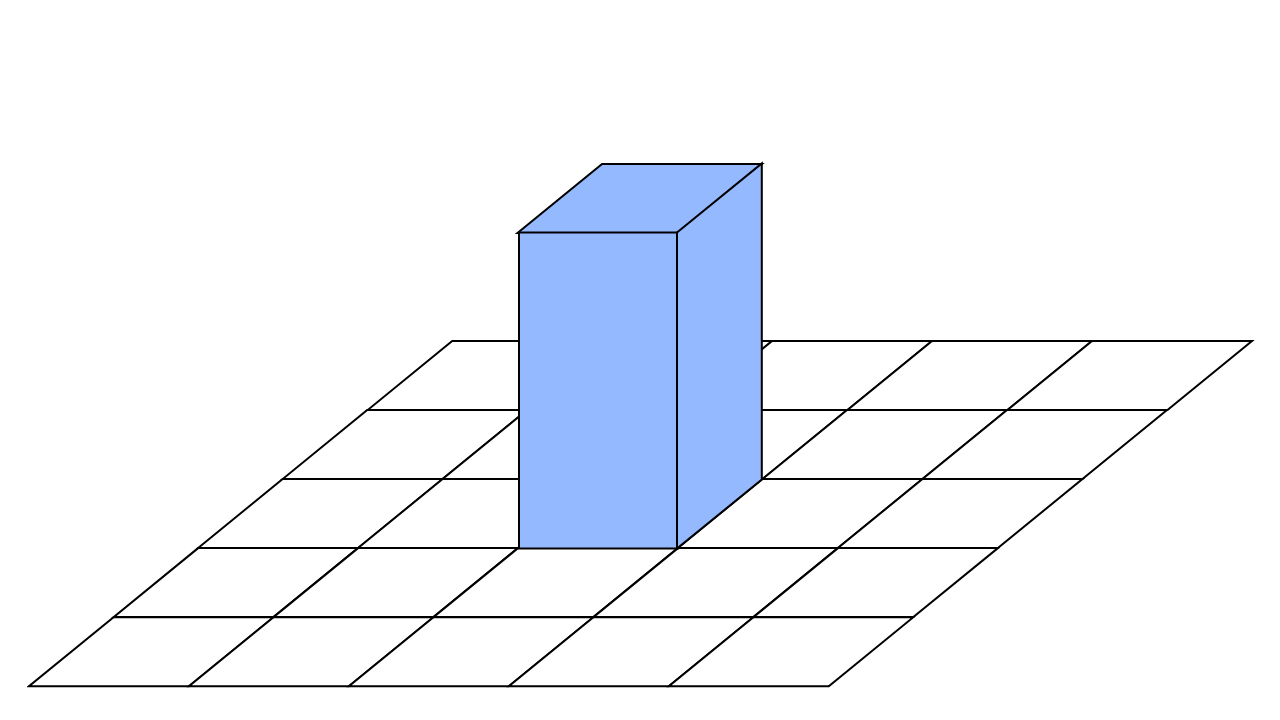
\includegraphics[width=120px]{balok-1-awal}
\end{center}

Maka balok dapat digulingkan menjadi salah satu dari berikut:

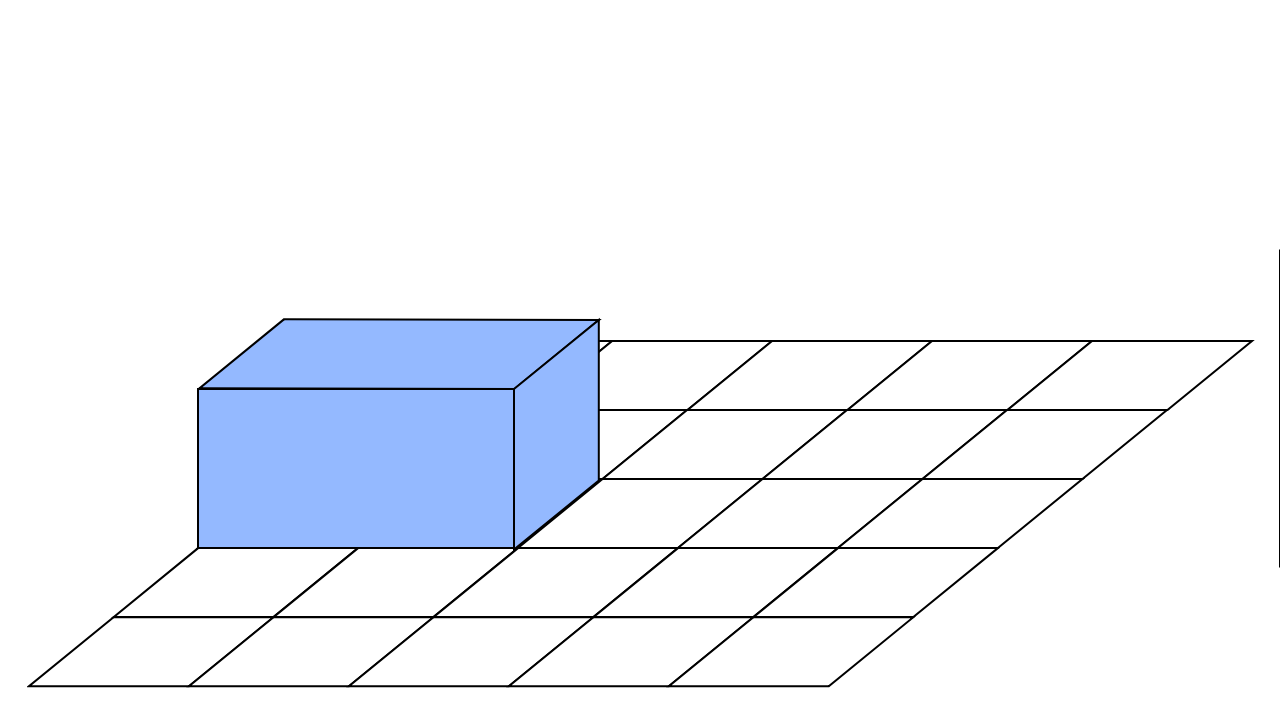
\includegraphics[width=120px]{balok-1-kiri}
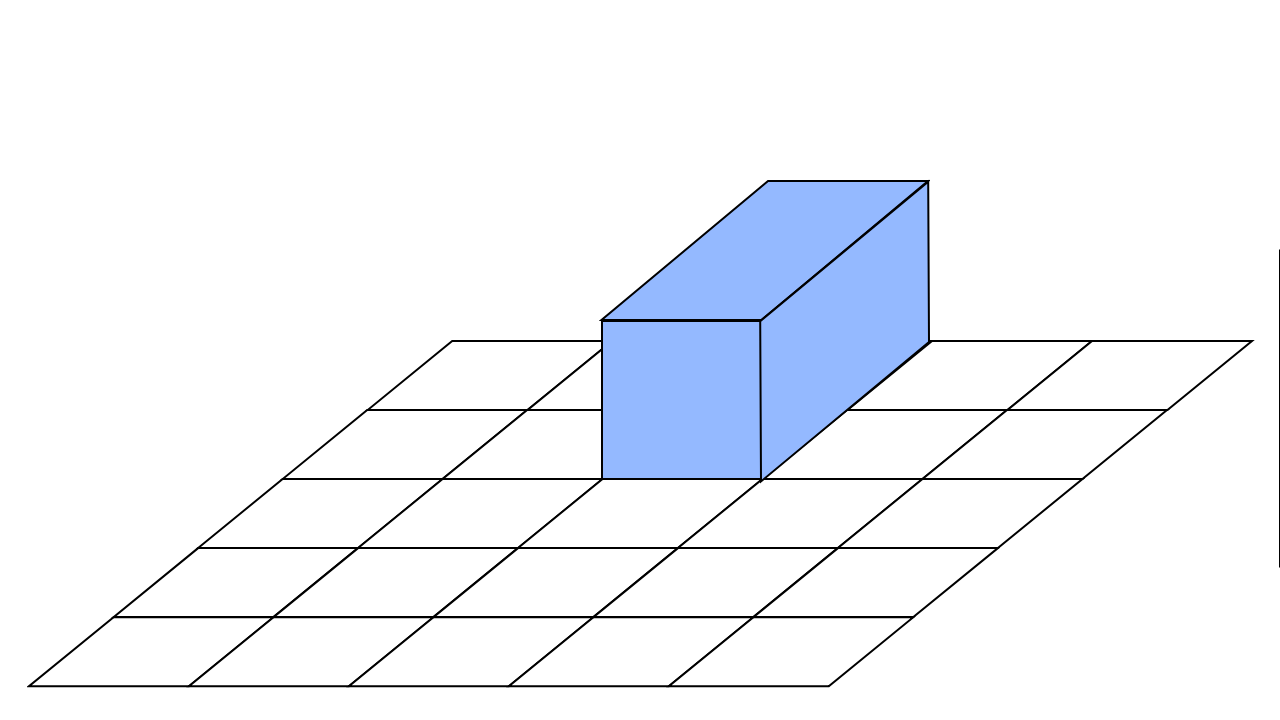
\includegraphics[width=120px]{balok-1-belakang}
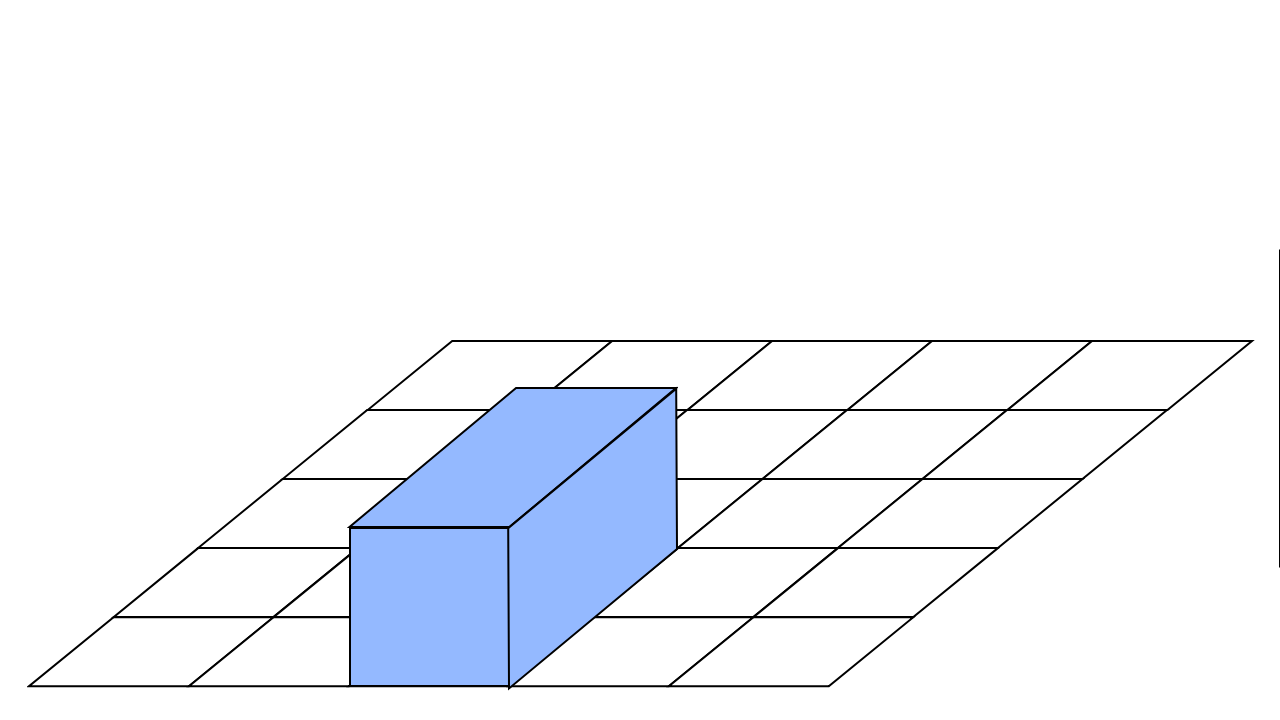
\includegraphics[width=120px]{balok-1-depan}
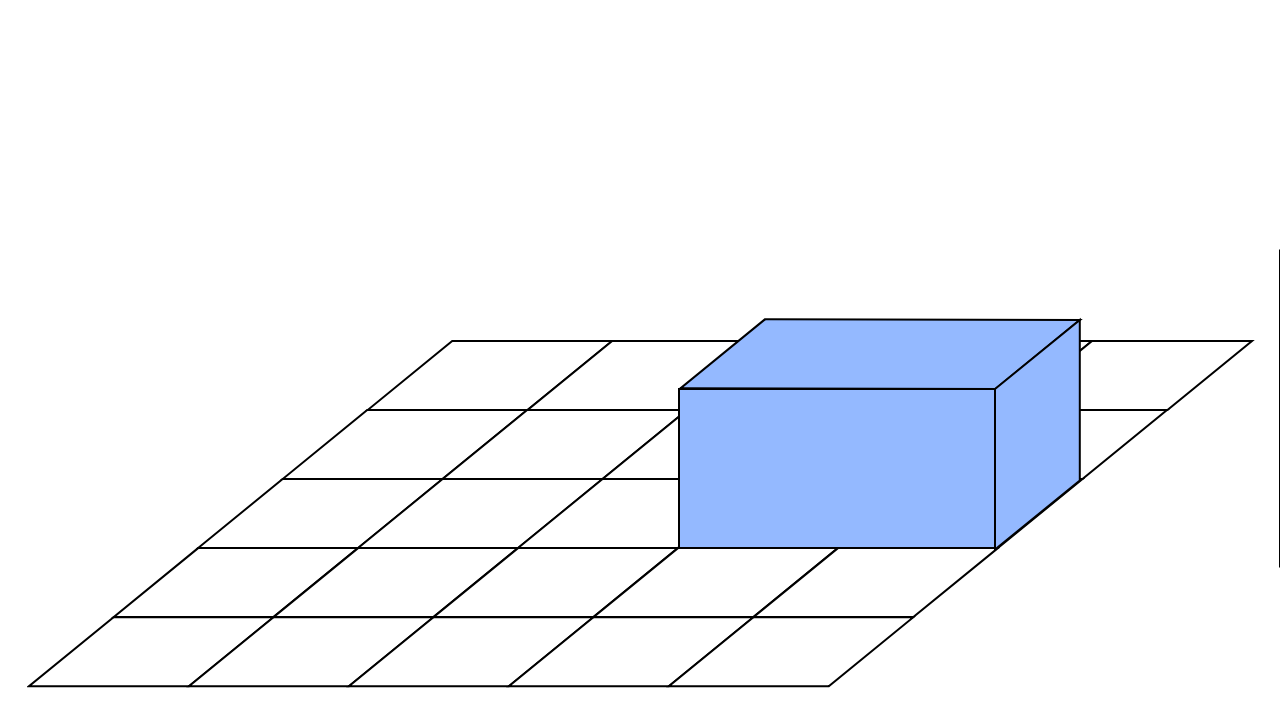
\includegraphics[width=120px]{balok-1-kanan}

Sedangkan ika balok besi berada pada posisi seperti ini:

\begin{center}
    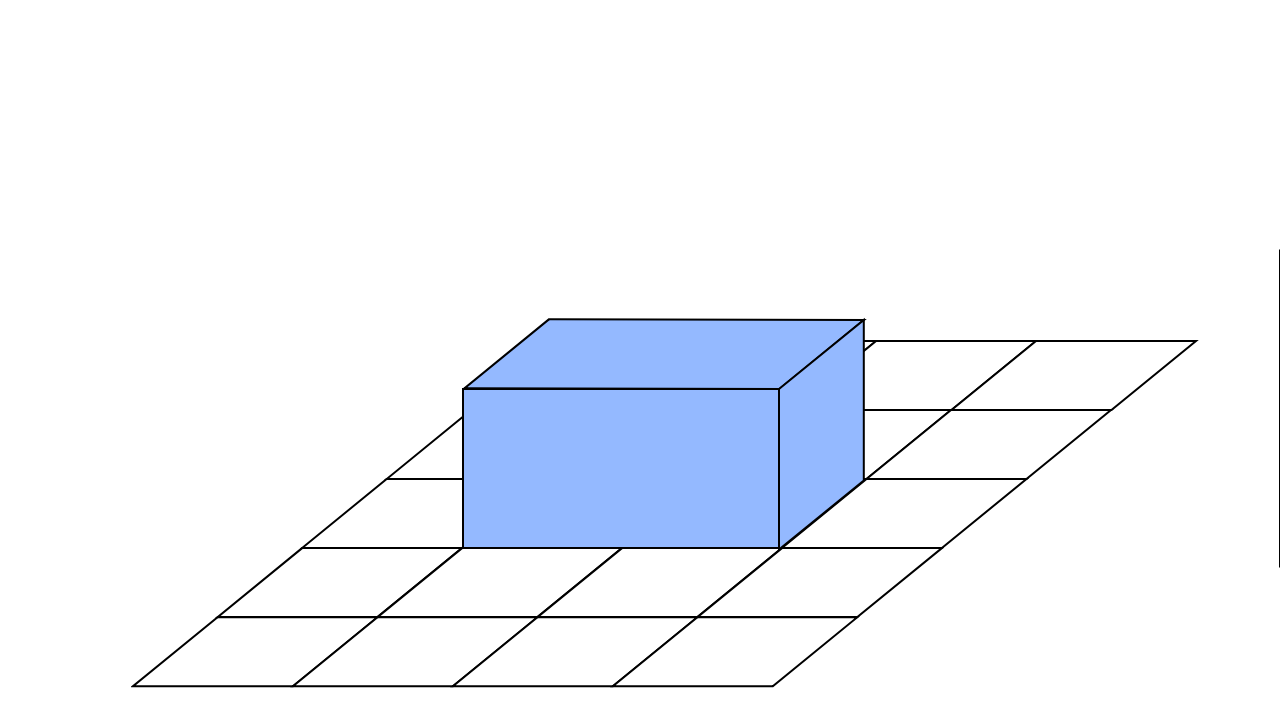
\includegraphics[width=120px]{balok-2-awal}
\end{center}

Maka balok dapat digulingkan menjadi salah satu dari berikut:

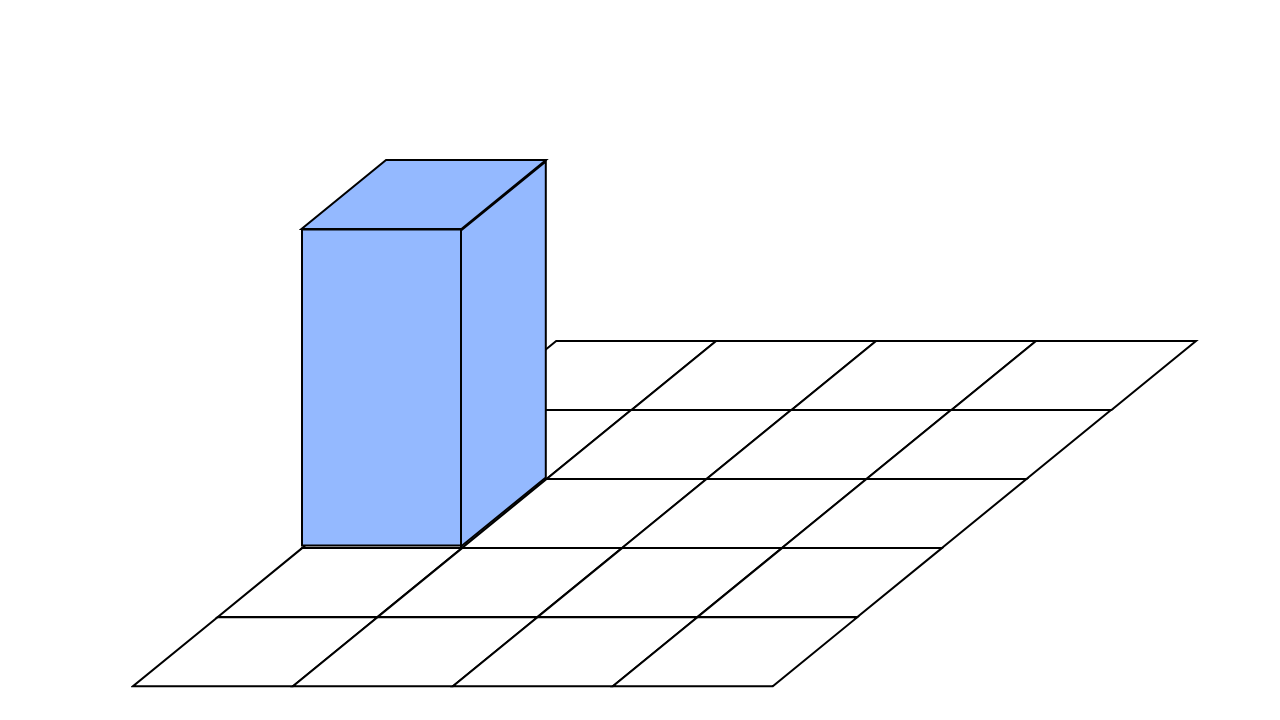
\includegraphics[width=120px]{balok-2-kiri}
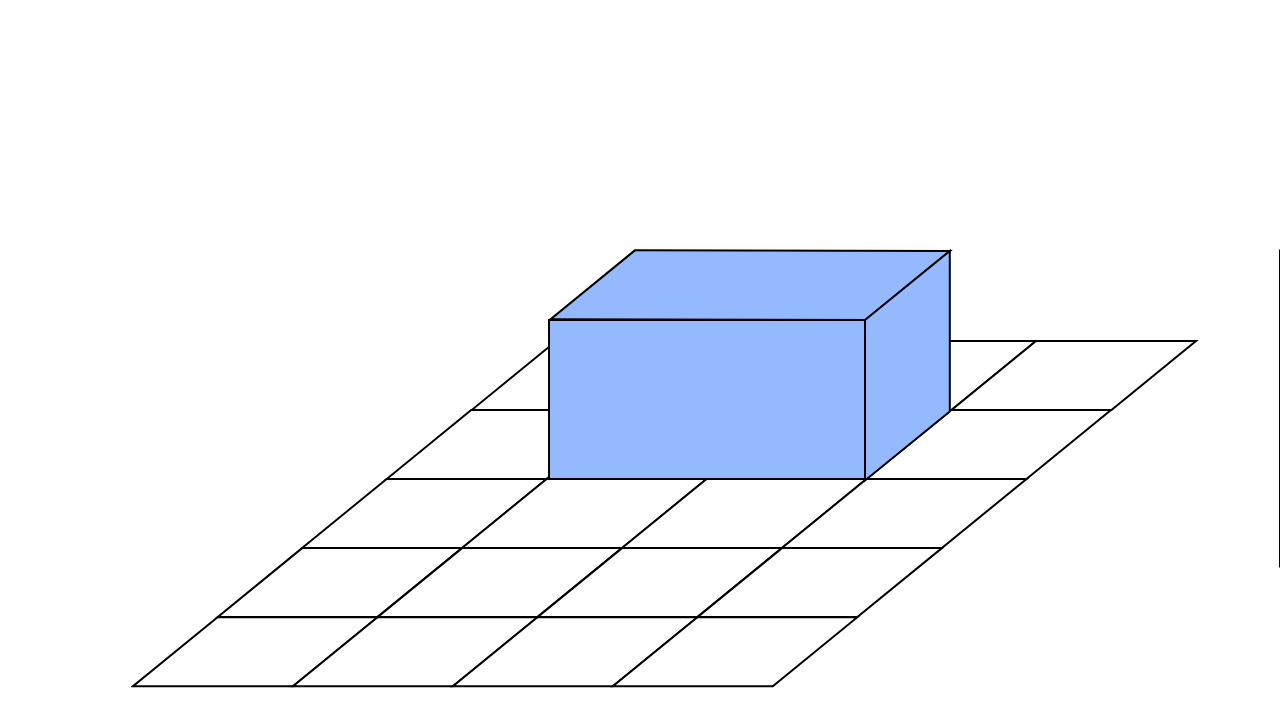
\includegraphics[width=120px]{balok-2-belakang}
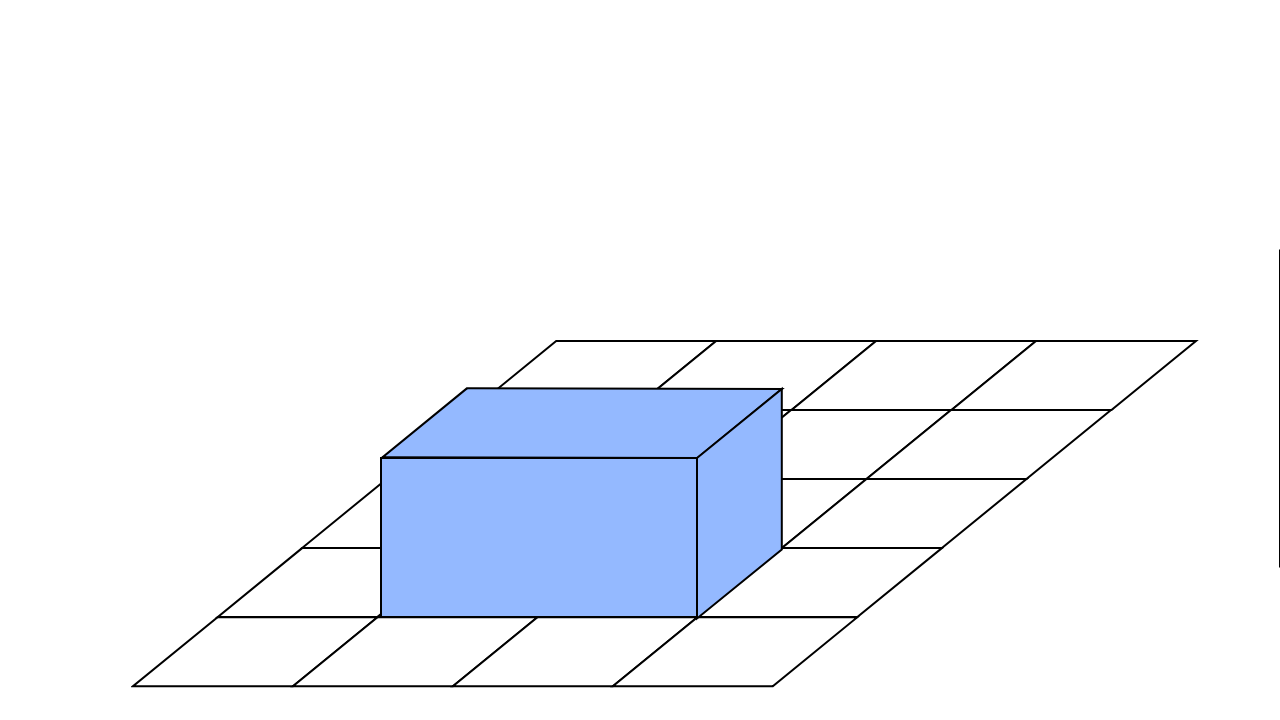
\includegraphics[width=120px]{balok-2-depan}
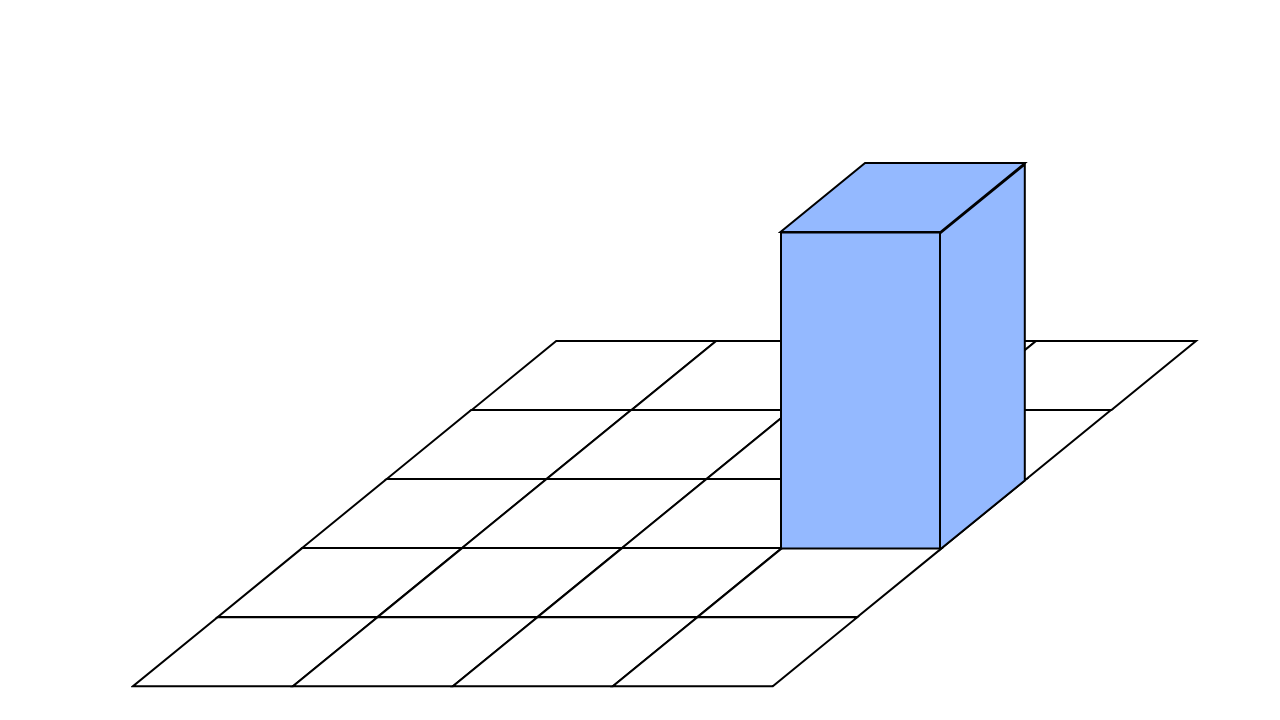
\includegraphics[width=120px]{balok-2-kanan}

Buatlah program yang dapat membantu Arvy menghitung rute terpendek untuk memindahkan balok besi dengan cara tersebut.

\pagebreak

\subsection*{Format Masukan}
Baris pertama terdiri dari satu bilangan bulat positif $T$ ($1 \leq T \leq 100$), menyatakan banyaknya kasus uji.
Tiap kasus uji dimulai dengan sebuah baris berisikan bilangan bulat $R$ dan $C$ ($3 \leq R, Q \leq 100$).

$R$ baris berikutnya terdiri dari $C$ buah karakter, menggambarkan gudang. Jika karakter berupa:
\begin{itemize}
    \setlength\itemsep{0pt}
    \item titik (\lstinline{.}), artinya balok bisa berada di kotak tersebut.
    \item pagar (\lstinline{#}), artinya ada halangan sehingga balok tidak bisa berada di kotak tersebut.
    \item karakter B (\lstinline{B}), artinya balok sedang berada di kotak tersebut.
    \item karakter F (\lstinline{F}), artinya balok harus berdiri di kotak tersebut.
\end{itemize}

Dijamin karakter F muncul tepat sekali, sedangkan karakter B bisa muncul satu atau dua kali. Jika sekali, artinya balok sedang berdiri di kotak tersebut. Jika dua kali, dijamin keduanya bersebelahan dan artinya balok sedang tertidur di kotak tersebut.

\subsection*{Format Keluaran}
Untuk tiap kasus uji, tuliskan sebuah baris menyatakan banyaknya langkah paling minimum untuk balok berdiri di karakter F. Jika balok tidak mungkin dipindahkan ke tujuan, tuliskan \lstinline{-1}
\\

\begin{multicols}{2}
\subsection*{Contoh Masukan}
\begin{lstlisting}
2
4 5
#...#
BB.#.
..F..
#....
6 6
......
.##.B.
.#....
F.....
...#..
#.....
3 3
BB.
.F.
...
\end{lstlisting}
\columnbreak
\subsection*{Contoh Keluaran}
\begin{lstlisting}
2
9
-1
\end{lstlisting}
\vfill
\null
\end{multicols}


\subsection*{Penjelasan}
Pada kasus uji pertama, langkah-langkah pergerakan balok akan seperti berikut:

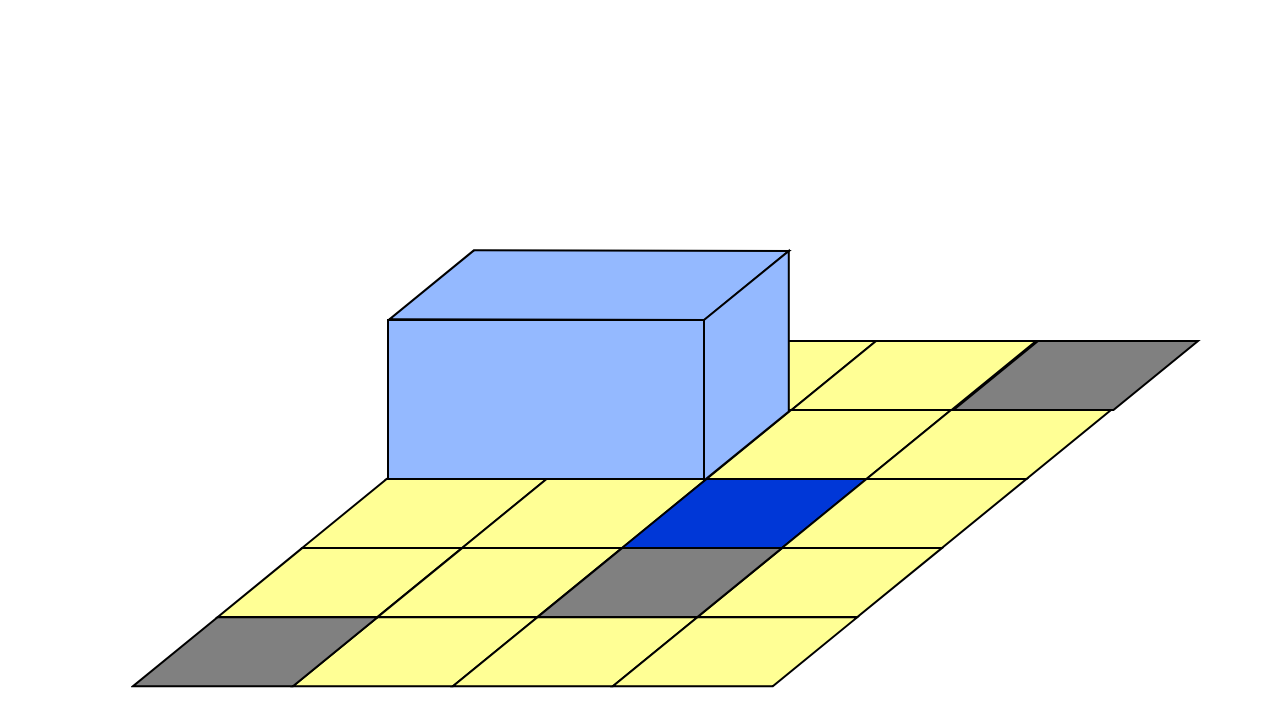
\includegraphics[width=120px]{sample-1-1}
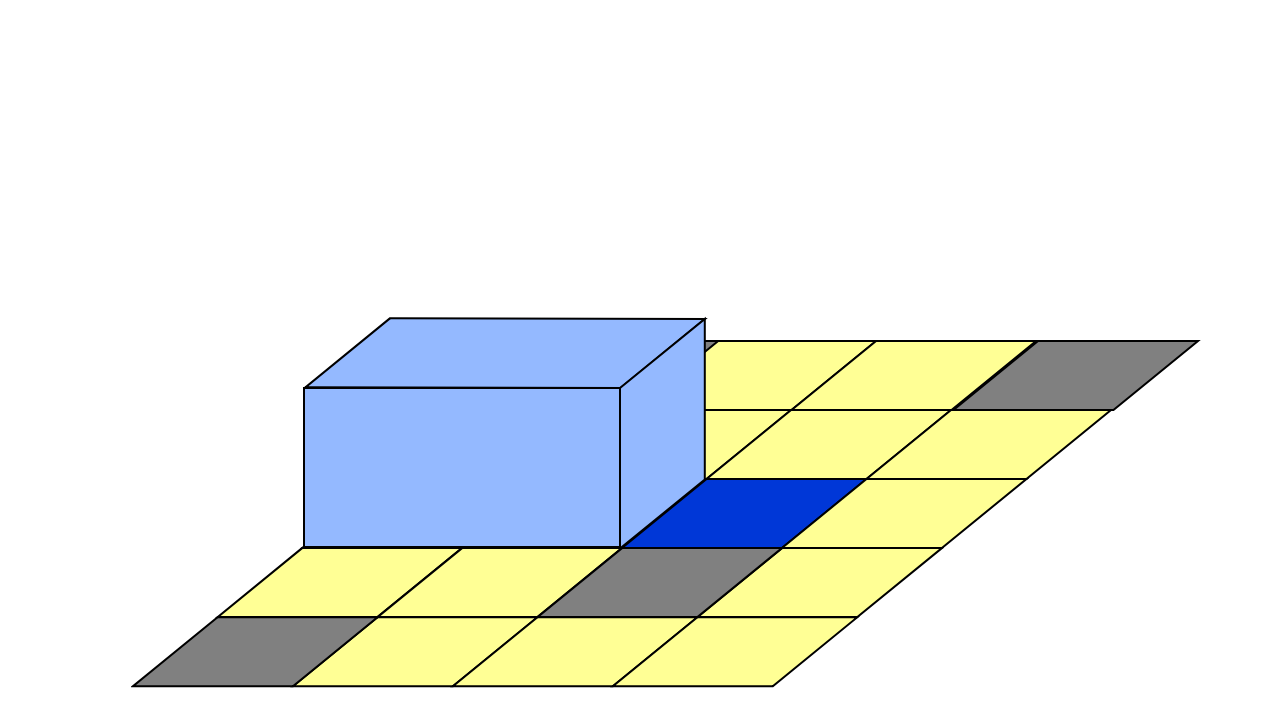
\includegraphics[width=120px]{sample-1-2}
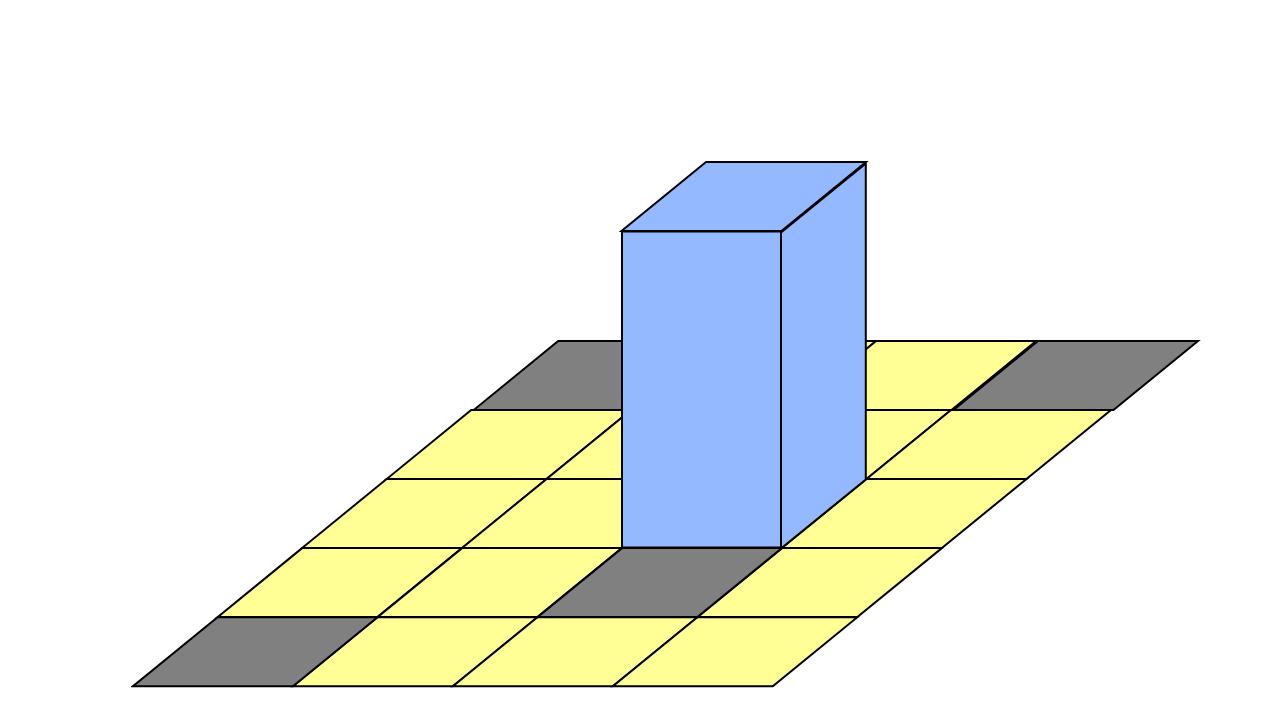
\includegraphics[width=120px]{sample-1-3}

\pagebreak
\end{document}
